
\begin{titlepage}
\chapter*{Pencak Silat Rules \& Regulations}
\begin{center}
    \begin{figure*}[ht!]
    \subfigure{
        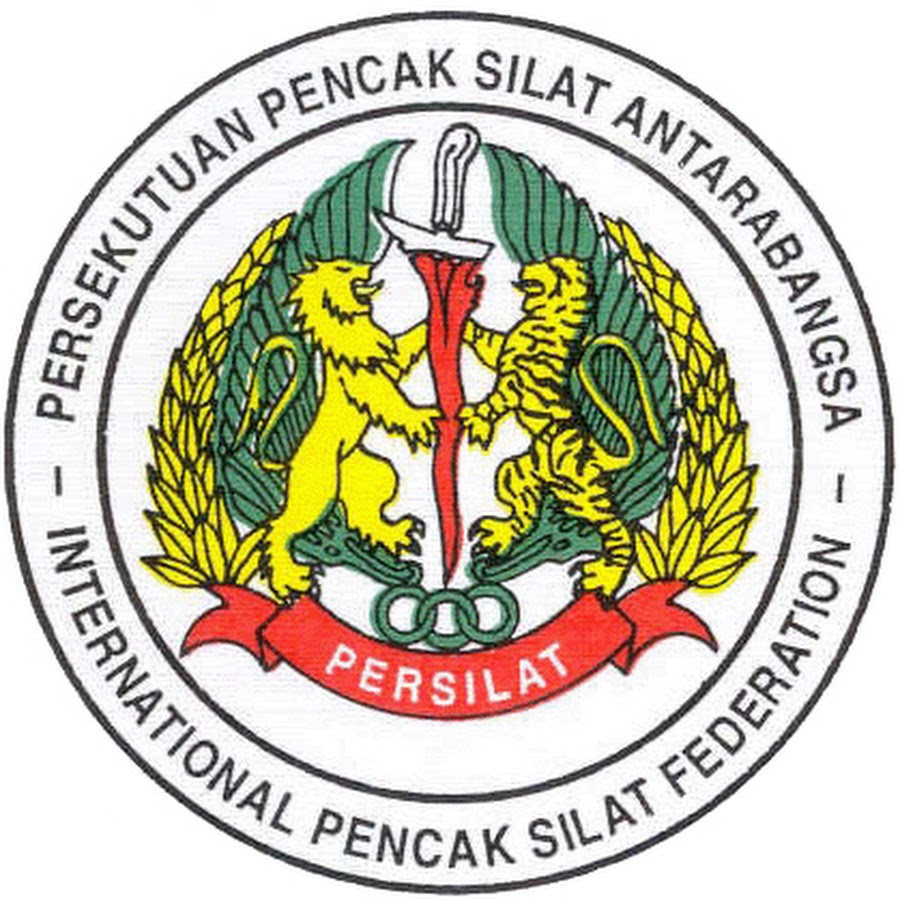
\includegraphics[height=2.75in]{images/persilat_logo}
    }
    ~
    \subfigure{
        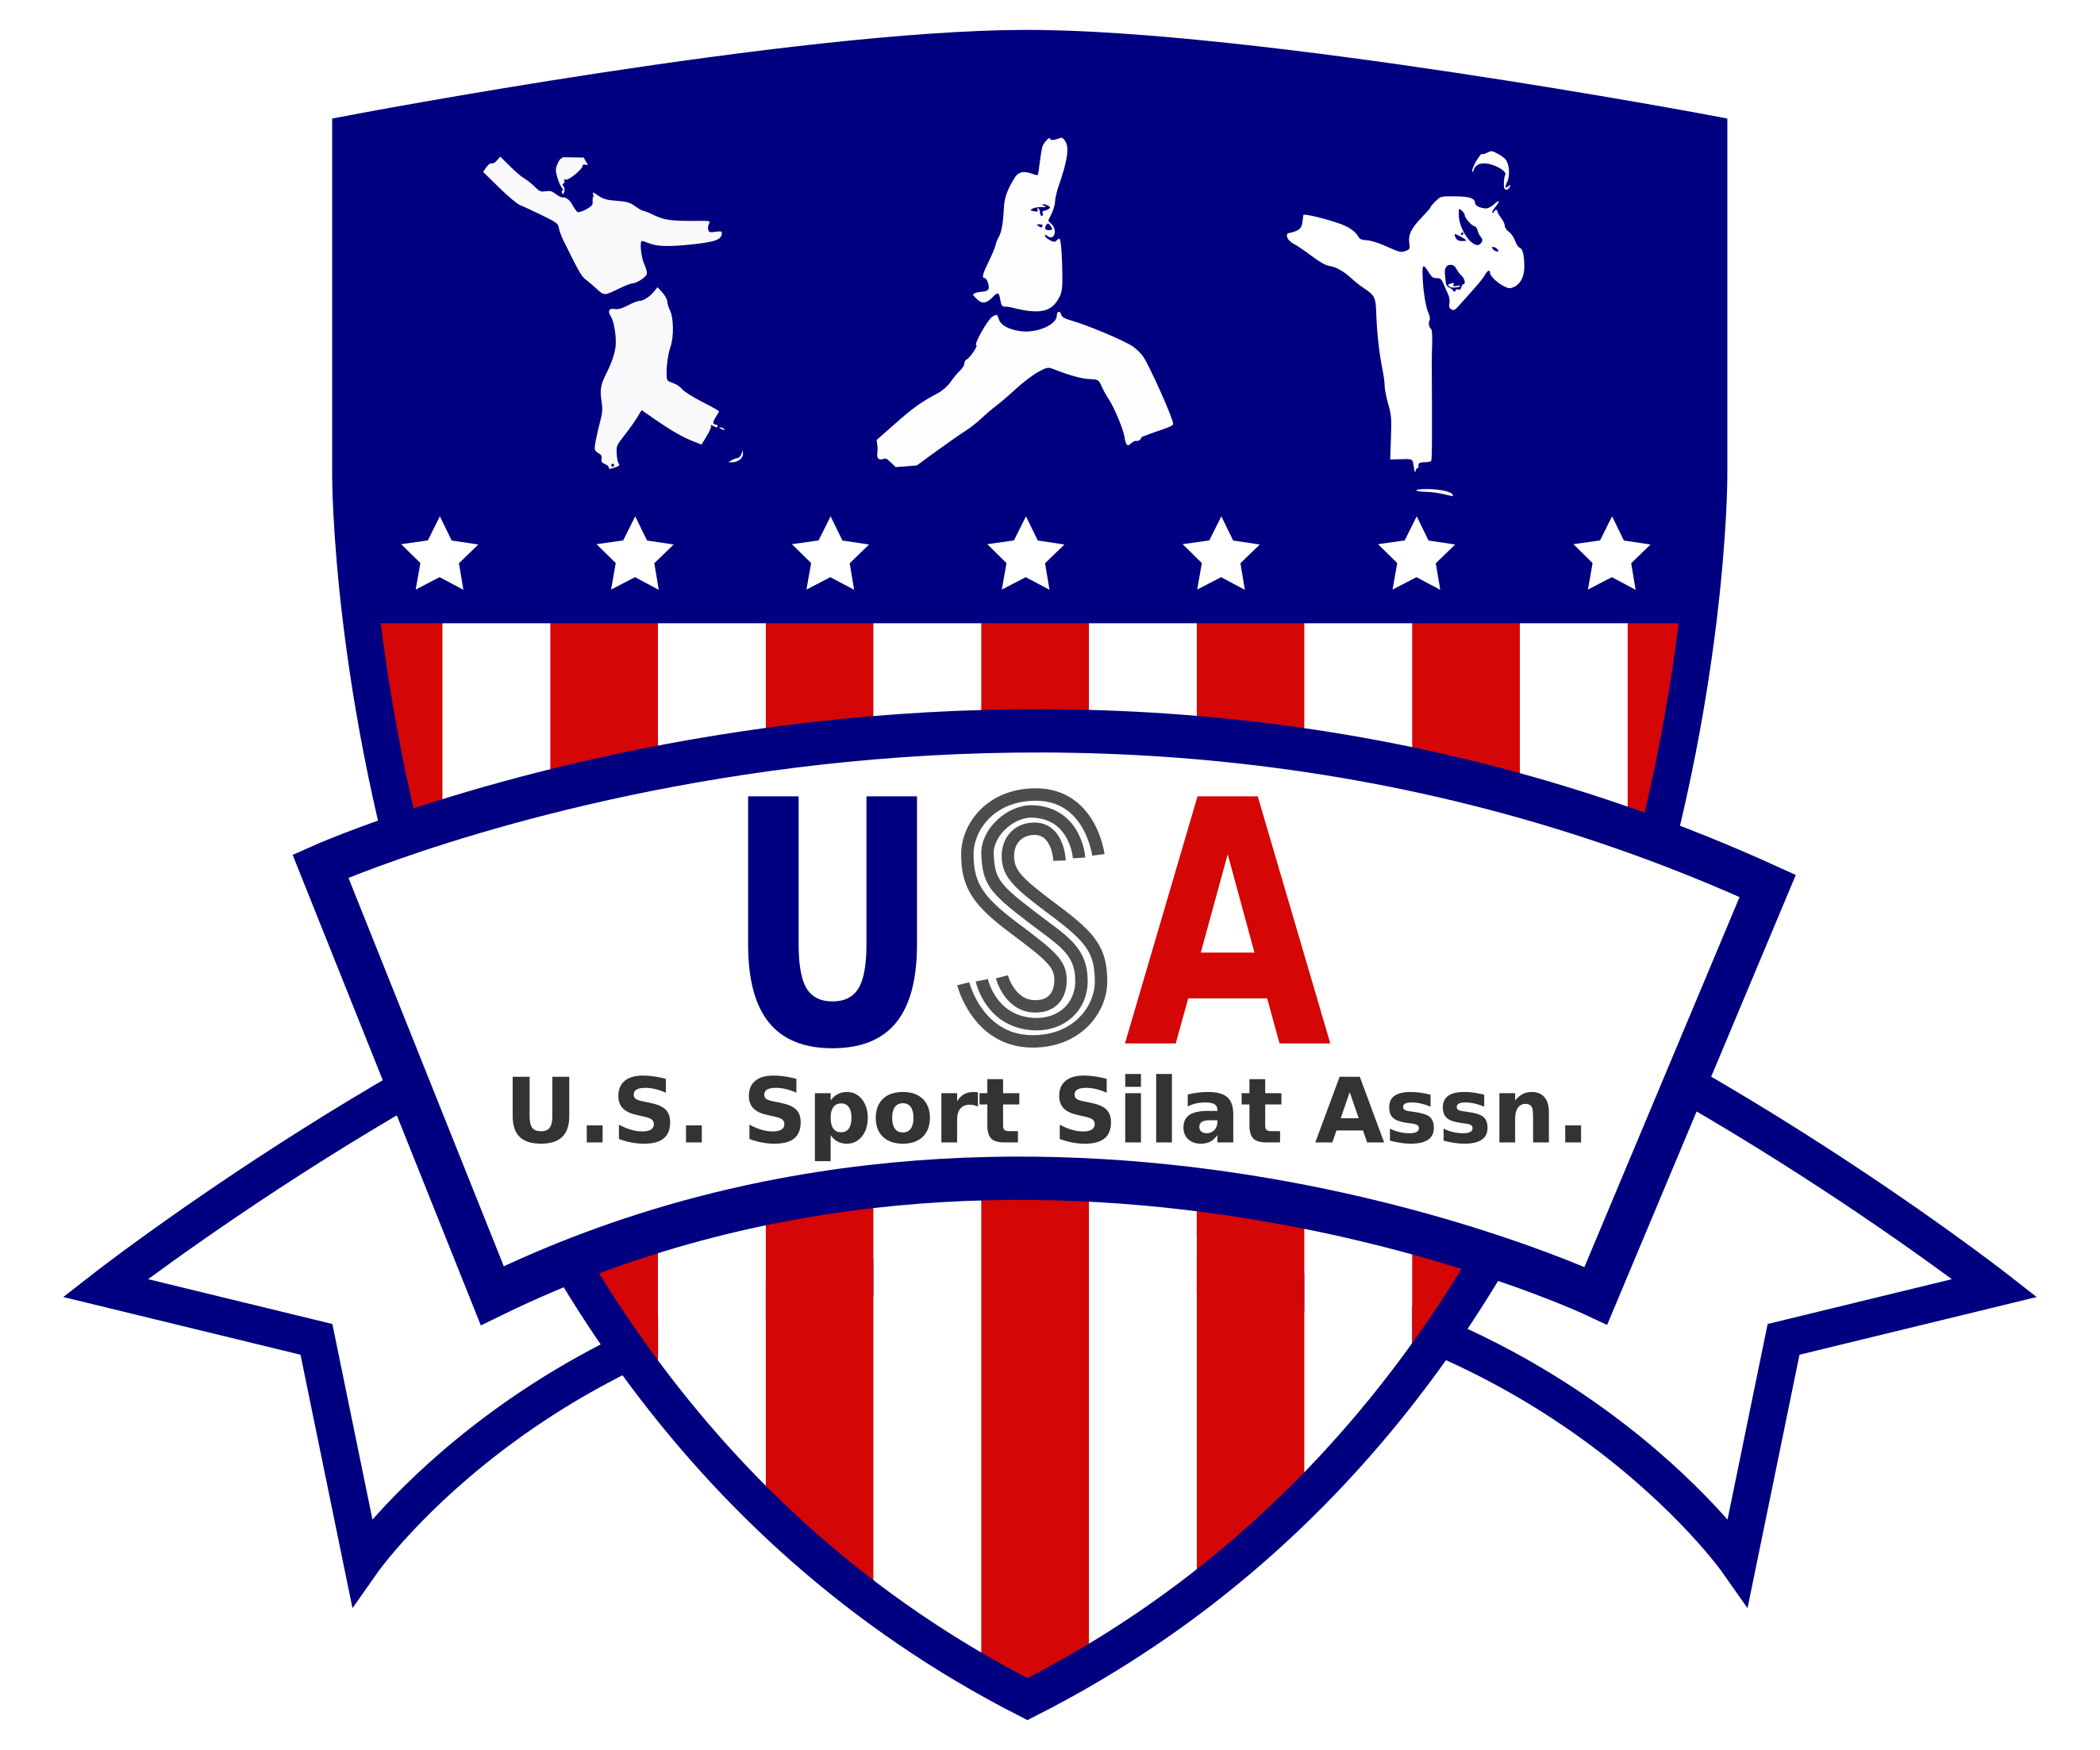
\includegraphics[height=2.75in]{images/USSSA_shield_white_border_300_dpi}
    }
\end{figure*}
\end{center}

\noindent International Pencak Silat Competitions are performed in principles of brotherhood and knightly soul by using elements of self defense, arts and Pencak Silat sports and by highly honoring the PESILAT PLEDGE.\\

\noindent The competitions are carried out in accordance with the category rules regulated in the competition regulations and conducted by certified legal and valid technical official of competitions. \\

\noindent Pencak Silat competition categories consist of: \\
\begin{enumerate}
    \item TANDING (Sparring Match) category
    \item TUNGGAL (Solo Performance) category
    \item GANDA (Choreographed Pair Performance) category
    \item REGU (Synchronized Team Performance) category
\end{enumerate}

\noindent In order to conduct Pencak Silat competition at the highest standards possible and in compliance with 
their intended purposes and objectives, the Pencak Silat Rules and Regulation is established as detailed in this technical manual.
\end{titlepage}

\section*{PERSILAT}
The governing body for international pencak silat is the International Pencak Silat Association or PERSILAT (Persekutuan Pencak Silat Antara Bangsa).

\begin{table*}
\begin{tabular}{p{3in}p{3in}}
\emph{A Pesilat is a person of noble character.\newline
A Pesilat is a person who respects his neighbor and loves friendship and peace.\newline
A Pesilat is a person who always thinks and acts positively, creatively and dynamically.\newline
A Pesilat is a knight who upholds truth, honesty and justice and always perseveres in facing temptations and trials.
\newline
A Pesilat is a knight who always takes responsibility for his words and actions.
}
&
\emph{Pesilat adalah pribadi yang berbudi pekerti luhur.\newline
Pesilat adalah insan yang menghormati sesamanya serta mencintai persaha-batan dan perdamaian.\newline
Pesilat adalah insan yang selalu berpikir dan bertindak positif, kreatif dan dinamis.\newline
Pesilat adalah kesatria yang menegakkan kebenaran, kejujuran dan keadilan serta senantiasa tahan uji dalam mengha-dapi godaan dan cobaan.\newline
Pesilat adalah kesatria yang senantiasa mempertanggungjawabkan kata-kata dan perbuatannya.
} \\
& \\
& --PERSILAT Pledge
\end{tabular}
\end{table*}

\section*{USSSA}

The United States Sport Silat Association (USSSA) is the sole national body for Pencak Silat competition in the United States recognized by the International Pencak Silat Federation (PERSILAT).

The USSSA coordinates local, state and national level competitions, so that it may field a strong USA Pencak Silat National Team that represents the United States' diversity of talent, knowledge and skill in Pencak Silat.

\subsection*{Mission}
To share the cultural heritage of Pencak Silat and the Indo-Malay archipelago with all Americans.

\subsection*{Vision}
To serve as a beacon of Pencak Silat values through sport, fellowship and education.  To bring together Pencak Silat players from all geographies and background.  To foster goodwill with other countries through competition and the shared bond of Pencak Silat.

